\def\year{2020}\relax
%File: formatting-instruction.tex
\documentclass[letterpaper]{article} % DO NOT CHANGE THIS
\usepackage{aaai20}  % DO NOT CHANGE THIS
\usepackage{times}  % DO NOT CHANGE THIS
\usepackage{helvet} % DO NOT CHANGE THIS
\usepackage{courier}  % DO NOT CHANGE THIS
\usepackage[hyphens]{url}  % DO NOT CHANGE THIS
\usepackage{graphicx} % DO NOT CHANGE THIS
\usepackage{subcaption}
\urlstyle{rm} % DO NOT CHANGE THIS
\def\UrlFont{\rm}  % DO NOT CHANGE THIS
\usepackage{graphicx}  % DO NOT CHANGE THIS
\frenchspacing  % DO NOT CHANGE THIS
\setlength{\pdfpagewidth}{8.5in}  % DO NOT CHANGE THIS
\setlength{\pdfpageheight}{11in}  % DO NOT CHANGE THIS
%\nocopyright
%PDF Info Is REQUIRED.
% For /Author, add all authors within the parentheses, separated by commas. No accents or commands.
% For /Title, add Title in Mixed Case. No accents or commands. Retain the parentheses.
 \pdfinfo{
/Title (Maximização de pontuação no jogo Freeway utilizando os algoritmos de aprendizado por reforço Proximal Policy Optimization (PPO) e Deep Q-Learning (DQN))
/Author (Vinicius Alves Matias)
} %Leave this	
% /Title ()
% Put your actual complete title (no codes, scripts, shortcuts, or LaTeX commands) within the parentheses in mixed case
% Leave the space between \Title and the beginning parenthesis alone
% /Author ()
% Put your actual complete list of authors (no codes, scripts, shortcuts, or LaTeX commands) within the parentheses in mixed case. 
% Each author should be only by a comma. If the name contains accents, remove them. If there are any LaTeX commands, 
% remove them. 

% DISALLOWED PACKAGES
% \usepackage{authblk} -- This package is specifically forbidden
% \usepackage{balance} -- This package is specifically forbidden
% \usepackage{caption} -- This package is specifically forbidden
% \usepackage{color (if used in text)
% \usepackage{CJK} -- This package is specifically forbidden
% \usepackage{float} -- This package is specifically forbidden
% \usepackage{flushend} -- This package is specifically forbidden
% \usepackage{fontenc} -- This package is specifically forbidden
% \usepackage{fullpage} -- This package is specifically forbidden
% \usepackage{geometry} -- This package is specifically forbidden
% \usepackage{grffile} -- This package is specifically forbidden
% \usepackage{hyperref} -- This package is specifically forbidden
% \usepackage{navigator} -- This package is specifically forbidden
% (or any other package that embeds links such as navigator or hyperref)
% \indentfirst} -- This package is specifically forbidden
% \layout} -- This package is specifically forbidden
% \multicol} -- This package is specifically forbidden
% \nameref} -- This package is specifically forbidden
% \natbib} -- This package is specifically forbidden -- use the following workaround:
% \usepackage{savetrees} -- This package is specifically forbidden
% \usepackage{setspace} -- This package is specifically forbidden
% \usepackage{stfloats} -- This package is specifically forbidden
% \usepackage{tabu} -- This package is specifically forbidden
% \usepackage{titlesec} -- This package is specifically forbidden
% \usepackage{tocbibind} -- This package is specifically forbidden
% \usepackage{ulem} -- This package is specifically forbidden
% \usepackage{wrapfig} -- This package is specifically forbidden
% DISALLOWED COMMANDS
% \nocopyright -- Your paper will not be published if you use this command
% \addtolength -- This command may not be used
% \balance -- This command may not be used
% \baselinestretch -- Your paper will not be published if you use this command
% \clearpage -- No page breaks of any kind may be used for the final version of your paper
% \columnsep -- This command may not be used
% \newpage -- No page breaks of any kind may be used for the final version of your paper
% \pagebreak -- No page breaks of any kind may be used for the final version of your paperr
% \pagestyle -- This command may not be used
% \tiny -- This is not an acceptable font size.
% \vspace{- -- No negative value may be used in proximity of a caption, figure, table, section, subsection, subsubsection, or reference
% \vskip{- -- No negative value may be used to alter spacing above or below a caption, figure, table, section, subsection, subsubsection, or reference

\setcounter{secnumdepth}{0} %May be changed to 1 or 2 if section numbers are desired.

% The file aaai20.sty is the style file for AAAI Press 
% proceedings, working notes, and technical reports.
%
\setlength\titlebox{2.5in} % If your paper contains an overfull \vbox too high warning at the beginning of the document, use this
% command to correct it. You may not alter the value below 2.5 in
\title{Maximização de pontuação no jogo Freeway através de Aprendizado por Reforço}
%Your title must be in mixed case, not sentence case. 
% That means all verbs (including short verbs like be, is, using,and go), 
% nouns, adverbs, adjectives should be capitalized, including both words in hyphenated terms, while
% articles, conjunctions, and prepositions are lower case unless they
% directly follow a colon or long dash
\author{Vinicius Alves Matias\textsuperscript{\rm 1} \\ 
\textsuperscript{\rm 1}Escola de Artes, Ciências e Humanidades da Universidade de São Paulo\\ %If you have multiple authors and multiple affiliations
% use superscripts in text and roman font to identify them. For example, Sunil Issar,\textsuperscript{\rm 2} J. Scott Penberthy\textsuperscript{\rm 3} George Ferguson,\textsuperscript{\rm 4} Hans Guesgen\textsuperscript{\rm 5}. Note that the comma should be placed BEFORE the superscript for optimum readability
Rua Arlindo Bettio, 1000, São Paulo/SP\\
viniciusmatias@usp.br % email address must be in roman text type, not monospace or sans serif
}

 \begin{document}

\maketitle

\begin{abstract}
A aplicação de algoritmos de Aprendizado por Reforço em diversos problemas do mundo real está sendo cada vez mais possível devido os avanços feitos na literatura da área, tendo essa área também uma particularidade que não é tão vista em outras ramificações de Aprendizado de Máquina: a utilização de jogos para avaliação do desempenho dos algoritmos. Neste artigo será discutida a aplicação de dois algoritmos publicados em há menos de 10 anos,  mas que em muitos casos permitem que um agente aprenda em uma ambiente sem nenhuma grande adaptação ao método original proposto. Os algoritmos de Aprendizado por Reforço analisados foram o Proximal Policy Optimation (PPO) e o Deep Q-Learning Network (DQN). Para uma análise em um ambiente discretizado foram usados os algoritmos Value Iteration (VI) e Policy Iteration (PI). O jogo do Atari escolhido foi o Freeway, tendo este um ponto específico de recompensas esparsas. 
\end{abstract}

\section{Introdução}
Freeway é um jogo desenvolvido pela Activision e disponibilizado para o Atari 2600 (Activision 1981). O objetivo é fazer uma galinha atravessar uma via expressa enquanto desvia de veículos, acumulando um ponto ao atravessar todas as faixas sem ser atingida. Quando a galinha encontra um carro, ela volta duas posições com um delay curto, podendo ser atingida por outros carros nesse período. A pontuação máxima atingida até o momento neste jogo foi de 34 pontos (Tang et al 2017), por meio do algoritmo \textit{TRPO-hash}.

\begin{figure}[h]
\centering
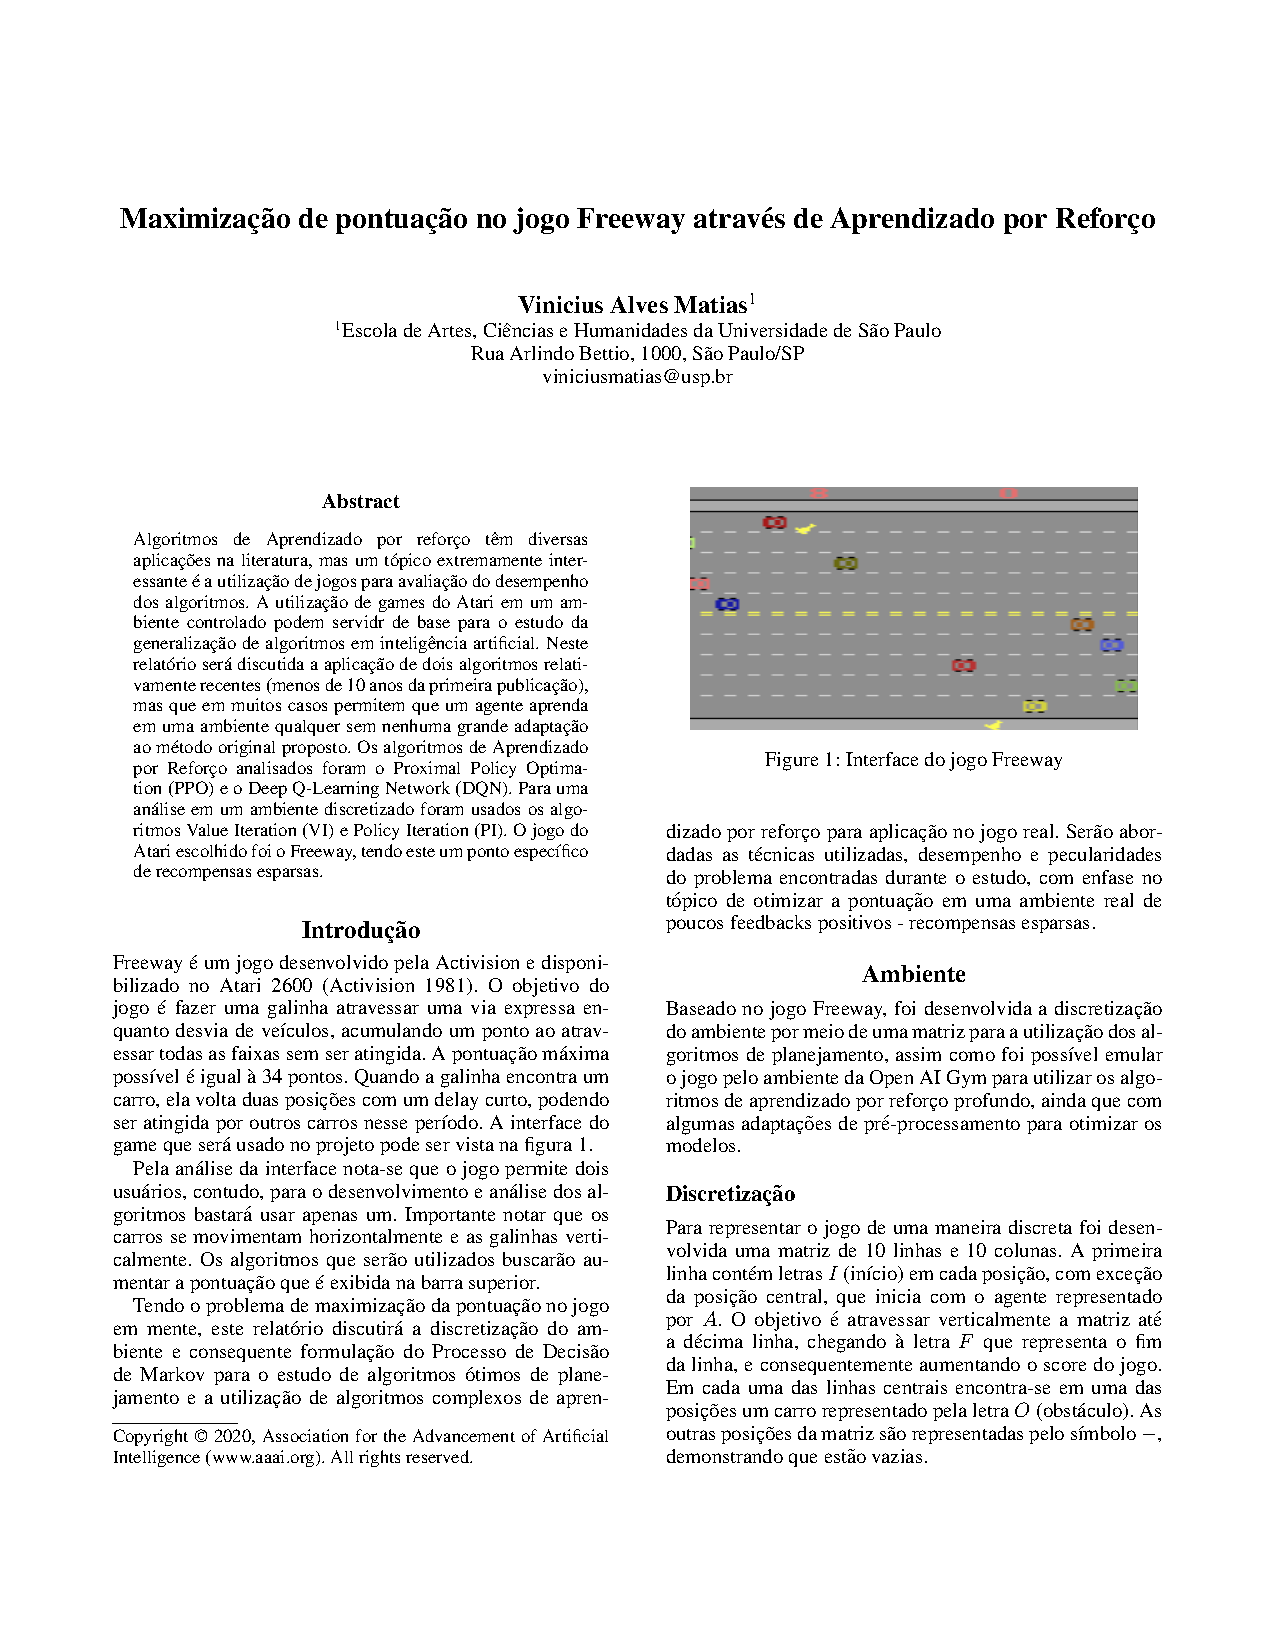
\includegraphics[width=0.7\columnwidth]{freeway.png}
\caption{Interface do jogo Freeway}
\label{fig:freeway}
\end{figure}

Pela análise da interface da figura \ref{fig:freeway} nota-se que o jogo permite dois usuários, contudo, para o desenvolvimento e análise dos algoritmos bastará usar apenas um. Importante notar que os carros se movimentam horizontalmente e as galinhas verticalmente. Os algoritmos que serão utilizados buscarão aumentar a pontuação que é exibida na barra superior.

Tendo o problema de maximização da pontuação no jogo em mente, este artigo discutirá a discretização do ambiente e consequente formulação do Processo de Decisão de Markov para o estudo de algoritmos ótimos de planejamento e a utilização de algoritmos complexos de aprendizado por reforço para aplicação no jogo real. Serão abordadas as técnicas utilizadas, desempenho e pecularidades do problema encontradas durante o estudo, com ênfase no tópico de otimizar a pontuação em uma ambiente real de poucos feedbacks positivos.

\section{Ambiente}
Baseado no jogo Freeway, foi desenvolvida a discretização do ambiente por meio de uma matriz para a utilização dos algoritmos de planejamento, assim como foi possível emular o jogo pelo ambiente da Open AI Gym (Brockamn et al 2016) para utilizar os algoritmos de aprendizado por reforço profundo.

\subsection{Discretização}
Para representar o jogo de uma maneira discreta foi desenvolvida uma matriz de 10 linhas e 9 colunas. A primeira linha contém letras $I$ (início) em cada posição, com exceção da posição central, que inicia com o agente representado por $A$. O objetivo é atravessar verticalmente a matriz até a décima linha, chegando à letra $F$ que representa o fim da linha, e consequentemente aumentando o score do jogo. Em cada uma das linhas centrais encontra-se em uma das posições um carro representado pela letra $O$ (obstáculo), inserido de forma aleatória. As outras posições da matriz são representadas pelo símbolo $-$, demonstrando que estão vazias. 

Como o jogo tem um tempo limite de 136 segundos (Weiss 2007), o ambiente também terá um tempo delimitado especificado. Para este artigo segue-se que haverão 272 iterações (uma referência à possibilidade ocorrem duas mudanças no ambiente por segundo), isto é, para cada iteração $t$ o agente poderá tomar uma ação, assim como os carros se moverão para a próxima posição válida na sua linha - à esquerda ou na primeira posição à direita quando chega ao limite da matriz. Para o ambiente discreto não foi considerada uma velocidade específica para cada veículo, mas sim uma mesma para todos. A figura 2 exemplifica essa mudança do ambiente para uma próxima iteração. A transição de um estado para outro atualiza o ambiente, tal como os veículos.

\begin{figure}[h]
     \begin{subfigure}[h]{0.2\textwidth}
         \centering
         \includegraphics[width=\textwidth]{discreto_t1.png}
         \caption{Ambiente em $t$}
     \end{subfigure}
     \hfill
     \begin{subfigure}[h]{0.2\textwidth}
         \includegraphics[width=\textwidth]{discreto_t2.png}
         \caption{Ambiente em $t+1$}
     \end{subfigure}
        \caption{Matriz que representa o ambiente discreto em um momento $t$ (a) e $t+1$ (b)}
\end{figure}

\subsection{Pré-Processamento no Atari}
Pelo ambiente de emulação do Atari (Bellemare et al 2013), a velocidade para execução de algoritmos que têm relação à redes neurais muitas vezes é dependente da entrada recebida. Para otimizar os algoritmo DQN foi realizado um redimensionamento nos frames enviados aos jogos. A dimensão de 210px (altura) por 160px (largura) passou para 84X84. Esse redimensionamento influenciou em uma redução de 34 milhões de parâmetros possíveis na rede neural para 5 milhões.

\subsection{Recompensas esparsas}
Em planejamento, quando discretizamos o ambiente podemos facilmente determinar recompensas para incentivar o aprendizado de um agente. Isso implica que não teremos apenas recompensas positivas, mas também negativas facilmente detectáveis.

Em ambientes reais, contudo, a definição das recompensas deve estar atrelada ao que se tem disponível do ambiente, e por vezes essa recompensa não é frequente. Ambientes desse tipo se enquadram no problema de recompensas esparsas (Hare 2019).

\textit{Freeway} tem apenas uma recompensa bem definida, que é chegar ao fim da via expressa (aumentar o score do jogo em 1). Para adquirir essa recompensa, contudo, o agente deve passar por todos os obstáculos e então receber o feedback.

Isso não é tão incomum em jogos do Atari, tanto que os algoritmos PPO e DQN tentam contornar esses problemas por intermédio de um certo controle de aleatoriedade - nem sempre utilizar a melhor ação para um estado, que tipicamente seria a de ficar confortável sem receber nenhuma recompensa

Ainda que para o \textit{Freeway} as recompensas esparsas não sejam muito problemáticas, em alguns problemas pode ser mais interessante buscar algoritmos que buscam explorar muito o ambiente em busca de informações que possam ser úteis posteriormente, isto é, algoritmos que "dirigidos à curiosidade" (Pathak et al. 2017) , que possivelmente teriam desempenho decente sob o jogo em questão.

\section{Markov Decision Process}
O ambiente discretizado é a base para a aplicação dos algoritmos de planejamento, que são úteis para analisar o comportamento do problema em um ambiente controlado. Antes de iniciar esse estudo, note que no ambiente discreto temos 9 posições possíveis para o agente (chegar ao estado meta implica retornar à posição inicial) e 272 iterações, assim, a máxima pontuação possível será de $\lceil \frac{272}{9}\rceil = 31$ pontos. Com isto dito, podemos definir o MDP (\textit{Markov Decision Process}), que podese ser definido como uma tupla $<S,A,D,T,R>$ (Mausam and Kolobov, 2012), onde: 

\begin{itemize}

\item $s \in S$ são os estados. O agente explora uma sequência de 10 estados (tendo no máximo três visíveis diretamente) e cada um, por sua vez, leva informações coluna adjacente ao agente (de onde vêm os obstáculos). Note que o estado inicial $s_0$ é fixo e há um conjunto de estados metas $G$ (posição final da matriz) em que o agente chega ao fim da via expressa. Havendo então a possibilidade de um agente transitar em 10 estados (não se mantém no estado meta, mas transita para ele), e que cada estado pode ser ocupado por um obstáculo, agente ou espaço nulo com exceção do estado meta (que só pode ser ocupado pela referência de meta) e o estado inicial (que terá ou um agente ou espaço vazio), temos que existem $3^{10} + 1 + 2 = 59052$ composições de estado diferentes;

\item $a \in A$ são as ações, tendo um total de 3 possíveis no conjunto  $A = \{UP, DOWN, NOOP\}$;

\item $d \in D$ é o tempo (ou época) que ocorre a decisão, proveniente de um conjunto finito (não poderão ser mapeados estados inifinatamente);

\item $T$ é uma função de transição que mapeia o estado atual, época e ação em um estado $s_{t+1}$ para então atualizar o ambiente. A transição entre estados segue uma política derivada dos algoritmos, mas vale notar que a transição é determinista - não segue uma distribuição de probabilidade para definir qual estado ir;

\item $R$ é uma função de recompensa. Os algoritmos de planejamento entregam uma recompensa positiva igual à 1 para o estado meta, -1 para a colisão com os obstáculos, e nula para qualquer outra posição.

\end{itemize}

Problemas de Horizonte indeterminado englobam o conceito de estados meta, e de fato à um estado que o agente não sabe que deve chegar sem auxílio de um algoritmo. Esse ponto fica muito claro na necessidade de explorar o ambiente na fase de aprendizado por reforço até encontrar um \textit{score}. Em planejamento, podemos aproveitar o fato de delimitarmos o limite do processo (estado com recompensa positiva), e executar os algoritmos à partir dele como um algoritmo para Horizonte Finito.

Visto que queremos maximar a pontuação, devemos buscar uma política $\pi$ markoviana (decisão depende apenas do estado inicial em planejamento, apesar de poder se aproveitar de um \textit{buffer} com o histórico, em aprendizado por reforço), estacionária (não há uma relação entre tempo e transição/recompensa) e determinista (sempre será feita a mesma ação para uma configuração de estado).

\section{Algoritmos de Planejamento Probabilístico}
Esta seção visa trazer um embasamento teórico dos dois algoritmos ótimos para planejamento que serão utilizados nos experimentos.

\subsection{Value Iteration}
A Iteração de Valor (Sutton and Barto 2020) é um método usado em planejamento quando busca-se identificar qual estado de todo seu ambiente discreto é o que terá a melhor "recompensa" total, ou seja, maior valor. O Valor de cada estado é calculado mediante a aplicação do princípio de otimilidade de \textit{Bellman} para a incerteza de um ambiente (O'Donoghue et al 2018). Independente do estado inicial que se aplica a equação de Bellman, este deverá identificar o valor ótimo para no ambiente. A função valor ótima $V^{*}(s, n)$ para um estado $s$ em um passo $n$ de um problema de Horizon Finito é dada pela equação 1:

\begin{equation}
V^{*}(s, n) = \max_{a \in A} \ \{ R(s,a) + \sum_{s' \in S} T(s,a,s')  V(s', n-1)\}
\end{equation}

Essa equação é aplicada no problema de maneira recursiva à partir do estado meta do ambiente discretizado, e vai calculando o valor de todos os estados mediante a recompensa do estado $s'$ e a probabilidade de alcançá-lo com uma das três ações possíveis.

Como a iteração de valor não retorna uma política, é necessária uma adaptação ao método para, ao final, coletarmos a ação que proporcione o maior resultado para as ações possíveis em um estado $s$ (equação 2).

\begin{equation}
\pi(s, n) = arg \max_{a \in A} \ \{ R(s,a) + \sum_{s' \in S} T(s,a,s')  V(s', n-1)\}
\end{equation}


A recorrência permite a convergência do algoritmo à política ótima, mas ainda assim ele depende da definição de um ambiente que possa coletar alguma pontuação, caso contrário, pontuará zero. 

\subsection{Policy Iteration}
O algoritmo \textit{Value Iteration} retorna o valor ótimo para os estados de uma ambiente discreto, mas a política ótima para um estado deve ser computada após essa informação se seguirmos o algoritmo original proposto. O algoritmo \textit{Policy Iteration} visa suprir essa falta da obtenção da política ótima do \textit{Value Iteration}. Nesse algoritmo não itera-se a função valor, mas sim uma política inicial arbitrária (Sutton and Barto 2020).

Esse método de iteração consiste de duas partes essenciais: \textit{improvement} (melhoria) e \textit{evaluation} (avaliação). A fase de melhoria parte de uma política $\pi$ e aplica um algoritmo adaptado da forma de iteração de valor (equação 3).

\begin{equation}
V^{\pi}(s) = R(s,\pi(s)) + \sum_{s' \in S} T(s,\pi(s),s')  V^{\pi_i}(s')
\end{equation}

Essa equação pode ser vista como o valor de um estado $s$ pela política $\pi$ - inicializada com ações randomicas. Note que não usamos mais a ação de maneira pré-definida, mas uma ação proveniente da política que queremos melhorar.

A etapa de avaliação da política, por sua vez, recebe a função valor da política para calcular uma nova política $\pi'$ (equação 4).

\begin{equation}
\pi'(s) = arg \max_{a \in A} \ \{ R(s,a) + \sum_{s' \in S} T(s,a,s')  V^{\pi}(s')\}
\end{equation}

Executando essas iterações de política até a convergência, ou seja, $\pi = \pi'$. 

\section{Algoritmos de Aprendizado por Reforço}
Esta seção aborda também sob viés teórico, a estrutura dos algorimos de aprendizado por reforço profundo utilizados no \textit{Freeway}.

\subsection{Deep Q-Learning Network}
O algoritmo Deep Q-Learning Network foi proposto por uma equipe da DeepMind (Minth et al. 2013) em um artigo que ficou amplamente conhecido na área pela robustez do algoritmo. Tal como o nome sugere, esse algoritmo parte da definição do \textit{Q-Learning} (Szepesvári 2009).

\begin{equation}
Q(s,a) = R(s,a) + \gamma \max_{a \in A} Q(s',a)
\end{equation}

Na equação 5, $Q(s,a)$ é a soma da recompensa de se chegar em um estado $s$ com a ação $a$ somada ao próximo $Q(s',a)$ para uma ação $a$ que maximiza esse valor, descontada por um valor pré-definido $\gamma$. A recursão causada em $Q(s',a)$ é o que causa a convergência do \textit{Q-Learning}. É perceptível a aplicação da equação de \textit{Bellman} para gerar a convergência.

Pelo fato de a aplicação da recorrência não ser muito viável em problemas complexos e reais que o DQN propôs a adição de redes neurais com uma maneira de armazenar Q valores anteriores nesse problema.

A rede neural servirá para estimar o \textit{Q-value} para um estado e ação (com pesos aleatórios no início, mas se adaptando conforme o treinamento). O Q valor predito será comparado com o valor real de se tomar essa ação e, assim, podemos computar a perda na rede neural como o quadrado da diferença entre o predito e o retorno real. Um diferencial nesse processo é que armazena-se os últimos $n$ valores de Q para um um tupla estado-ação-estado predito, e durante a iteração da rede neural haverá uma probabilidade $1-\epsilon$ (alta no início) de tomarmos uma ação aleatória, mas que decresce no decorrer das iterações, e isso implica que tendemos à escolhermos uma ação que maximiza o \textit{Q-value} dentro da rede neural para um par estado-ação, mas com um probabilidade baixa de procurarmos outra ação.

Outro artigo publicado pela Deep Mind trazendo uma abordagem possível para treinamento de jogos no Atari (Mnih et al 2015), consistindo da utilização de redes convolucionais para tratar a entrada (e processá-la na rede) e por fim passá-la para uma camada profunda que terá como saída as ações possíveis de serem tomadas no jogo. Baseado neste artigo treinamos nosso agente em uma rede com a seguinte configuração: 

\begin{itemize}
	\item Uma entrada de frames 84X84X3 (3 canais);
	\item Uma camada oculta de 32 filtros 8X8 com stride 4 e função de ativação ReLU (convolucional);
	\item Uma camada oculta de 64 filtros 4X4 com stride 2 e função de ativação ReLU (convolucional);
	\item Uma camada oculta de 64 filtros 3X3 com stride 1 e função de ativação ReLU (convolucional);
	\item Uma camada \textit{Flatten} para intermediar as camadas convolucionais e densas
	\item Uma camada oculta de 512 perceptrons e função de ativação ReLU (densa)
	\item Uma camada oculta de 256 perceptrons e função de ativação ReLU (densa)
	\item Uma camada oculta de 3 perceptrons (quantidade de ações) e função de ativação ReLU (densa)
\end{itemize}

Onde filtro é o "tamanho" da janela em pixels que serão considerados, e \textit{strides} é em quantos pixels a janela será movimentada.

\subsection{Proximal Policy Optimization}
Problemas de apendizado por reforço profundo atribuem à redes neurais a tarefa de atuar como política em um ambiente, sendo seus neurônios de saída a melhor ação à ser tomada pelo que se tem conhecimento até então. Métodos \textit{Policy Gradient} seguem essa abordagem (Sutton et al 2000). Algoritmos dessa linha, como o \textit{Proximal Policy Optimization} (Schulman et al 2017) seguem uma abordagem mais conservadora para estimar o valor de um estado. 

O PPO é um algoritmo \textit{on-policy}, logo, aprende de acordo com a experiência atual do agente, e por isso precisam ter uma função \textit{Loss} à ser aplicada na rede neural que otimize as recompensas à serem obtidas, sendo definida para métodos de gradiente conforme a equação 6.

\begin{equation}
Loss^{PG}(\theta) =  \hat{E}_t[\log \pi_{\theta}(a_t | s_t) \hat{A}_t]
\end{equation}

Sendo ela basicamente é uma estimativa ($\hat{E}$) proveniente da multiplicação entre o logaritmo da probabilidade de se tomar uma ação $a$ em um estado $s_t$ pela política $\pi_{\theta}$ (a saída da rede neural) por uma estimativa Advantage $\hat{A}$. 

Existem várias maneiras de se calcular a estimativa \textit{Advantage}. Para a implementação deste artigo é utilizada a Generalized Advantage Estimation (GAE) descrita por Schulman et al (2018). Essa estimativa leva em conta o valor do estado predito pela rede neural (\textit{Critic}, como será visto na sequência) $V(s_{t+1})$, o valor do estado atual  $V(s_t)$, a recompensa real $r_t$ de se tomar a ação predita e chegar no estado previsto, e se esse estado é visível ($m_t$) no tempo $t$. Para evitar que se ocupe tempo demais nesse processamento, captura-se apenas as últimas 128 iterações armazenadas.

Dado o conhecimento das variáveis, o GAE pode ser calculado a partir da iteração mais recente em um \textit{loop} até a iteração armazenada mais antiga (de $t=127$ à $t=0$) performando as equações 7,8 e 9 na sequência. E Para gerar um escalar $\hat{A}$ foi considerado o desvio padrão de $Retornos_t(s_t, a_t)$, logo, $\hat{A} = \sigma(Retornos_t(s_t, a_t))$


\begin{equation}
\delta = r_t + \gamma V(s_{t+1}) m_t - V(s_t)
\end{equation}

\begin{equation}
gae_t = \delta + \gamma . \lambda . m_t . gae_{t+1}
\end{equation}

\begin{equation}
Retornos_t(s_t, a_t) = gae_t + V(s_t)
\end{equation}


A função \textit{Loss} é aplicada em um modelo \textit{Actor - Critic}, que resumidamente, consiste de dois modelos onde um gera uma saída (\textit{Actor}) e ou outro controla a variância dessa saída (\textit{Critic}). Uma maneira para evitar que enviesemos demais a função $Loss$ pela variância da estimativa \textit{Advantage} (algo bem comum quando utiliza-se a abordagem \textit{Actor-Critic}) é utilizando a política anterior para normalizar os resultados, consequentemente limitá-los, como visto naequação 10 (Schulman et al 2015).

\begin{equation}
r_t(\theta) = maximize_\pi \ \ \hat{E}_t \left[ \frac{\pi_{\theta}(a_t|s_t)}{\pi_{\theta_{old}}(a_t | s_t)} \hat{A} \right]
\end{equation}

Garantindo, portanto, que a política antiga não irá diferir muito da política atual. Finalmente, a função $Loss$ do PPO proposta em 2017 (equação 11) consiste da aplicação destes conceitos, além da adição de um corte entre valores para evitar mais ainda que a atualização de uma política não irá diferir muito de um momento para outro, ainda que influênciadas pelo valor de $\epsilon$ (neste artigo é 0.2).

\begin{equation}
L^{CLIP}(\theta) =  \hat{E}_t[min(r_t(\theta) \hat{A}_t, clip(r_t(\theta), 1 - \epsilon, 1 + \epsilon) \hat{A}_t)]
\end{equation}


\section{Experimentos e Resultados}
Esta seção discute os experimentos e resultados da aplicação dos quatro algoritmos estudados.

Importante notar que na aplicação dos algoritmos de planejamento alguns comportamentos que poderiam parecer à priori contraditórios ao método, são porém justificáveis pela composição do ambiente. Como mencionado na discretização do ambiente, os obstáculos são postos em posições aleatórias da matriz, e essa composição pode, em muitos casos, gerar um ambiente cujo agente não consiga chegar ao estado meta visto que cada estado inclui informações apenas da coluna adjacente às posições possíveis para deslocamente, justamente para reduzir a complexidade do método.

Optou-se por manter essa composição no ambiente discreto. A Activision, para evitar esse problema, inicializa, em toda a partida os agentes na mesma posição, mas com velocidades diferentes.

Para criar resultados que facilitem a comparação com algoritmos de aprendizado por reforço, cada \textit{frame} (instante t do ambiente desenvolvido) pode ser analisado como um ambiente discreto, ou seja, uma representação do jogo que pode ter algoritmos de planejamento probabilístico aplicáveis e, portanto, ter uma ação ótima de um estado para outro. Ao fim são esperadas $n\_epochs * 272$  aplicações do método de iteração de valor. 

Cada iteração de valor teve em média 300 equações de \textit{Bellman} executadas. A divergência na pontuação entre os jogos pode ser visto de maneira resumida pelo boxplot da figura \ref{fig:boxplot_vi}. Por ele é possível notar que uma pontuação maior que 15 é bem mais provável que uma menor.

\begin{figure}[h]
	\center
	\includegraphics[width=0.3\textwidth]{boxplot_vi.png}
    \caption{Execuções do Value Iteration. Cada intervalo compreende os scores finais em 120 ambientes de 10 estados.}
    \label{fig:boxplot_vi}
\end{figure}

\begin{figure}[h]
	\center
	\includegraphics[width=0.3\textwidth]{densidade_vi.png}
    \caption{Gráfico de densidade de probabilidade para os scores obtidos em 360 "jogos" executando Value Iteration. Cada jogo é composto por 272 iterações de valor seguidas em um ambiente de 10 estados.}
    \label{fig:densidade_vi}
\end{figure}


Como explicado neste tópico, o resultado um tanto quanto contra intuitivo de pontuações nulas mostrada nas figuras 3 e 4 tem uma explicação: a aleatoriedade da composição dos ambientes, e a sequência de ações ótima possível não necessariamente resultar em alcançar a meta.

Ainda assim, a maioria das pontuações finais foram maiores que 15 pontos, com a maior densidade nos valores entre 28 e 30 pontos (figura \ref{fig:densidade_vi}), implicando em uma média de 24.89 pontos. Vale notar que para atingir 31 pontos, os estados de maior valor deveriam sempre estar atrelados à ação de ir para frente, pois essa pontuação só é possível se, durante toda a execução do jogo, for possível ir para frente (após um longo período de treinamento, os algoritmos de aprendizado por reforço apresentam essa mesma tática, de ir sempre que possível à frente, mesmo que colidam com obstáculos e voltem duas casas).


O \textit{Policy Iterarion} teve um score médio de 23.83 em 360 jogos, que é próximo ao \textit{Value Iteration}, mas gerado atráves de comportamentos diferentes pelo agente atuando no ambiente. Na implementação do algoritmo, a convergência tipicamente demorou à ocorrer, e por isso delimitou-se um valor máximo de 100 iterações de política, caso não tenha convergido até então. Uma forte influência para o tempo foi a fase de avaliação da política. Nesse método o score final do jogo foi sempre de 0, 1, 30 ou 31 pontos, por isso um boxplot ou outro método de visualização dos dados conforme o tempo não são muito informativos.

\begin{figure}[h]
	\center
	\includegraphics[width=0.3\textwidth]{densidade_pi.png}
    \caption{Gráfico de densidade de probabilidade para os scores obtidos em 360 "jogos" executando Policy Iteration. Cada jogo é composto por 272 iterações de valor seguidas em um ambiente de 10 estados.}
    \label{fig:densidade_pi}
\end{figure}

Ainda que a maior parte dos jogos em 30 ou 31 pontos (Figura \ref{fig:densidade_pi}), na média o score cai para acompanhar os outros valores. Isso implica que o método escolhe a melhor ação para o conjunto de estados visível, mas não necessáriamente será a ação que, dada uma nova configuração do ambiente, resulte em uma otimização do resultado.

Em aprendizado por reforço foram relizados testes para diferentes valores de gamma $\gamma$, \textit{learning rate} $\alpha$, quantidade de épocas (jogos) mediante o número de passos, e tamanho do \textit{buffer} para analisar o DQN. Dois testes interessantes que sintetizam a ideia por trás do algoritmo aplicado no \textit{Freeway} serão mencionados aqui: ambos mantém o mesmo modelo sequêncial mencionado anteriormente, $\alpha = 0.01$ e $\gamma = 1$ incialmente (descrescendo até $\gamma = 0.1$. A diferença entre um teste e outro é dada pela quantidade de passos: o primeiro treinamento foi feito em 100 mil passos (mais de 36 jogos) e o segundo em 1 milhão de passos (mais de 360 jogos). A curva de aprendizado (aumento do \textit{score}) conforme aumenta a quantidade de passos pode ser vista na figura 6.

\begin{figure}[!h]
     \begin{subfigure}[h]{0.37\textwidth}
  	     \hspace{0.8cm}
         \includegraphics[width=\textwidth]{dqn_100k.png}
         \caption{100 mil passos}
     \end{subfigure}
     \hfill
     \begin{subfigure}[h]{0.37\textwidth}
	     \hspace{0.8cm}
         \includegraphics[width=\textwidth]{1M_dqn_passos.png}
         \caption{1 milhão de passos}
     \end{subfigure}
        \caption{Aumento na pontuação para 100 mil passos (a) e 1 milhão de passos (b) utilizando o algoritmo DQN}
\end{figure}

Vemos a mesma tendência nas duas curvas. Ambas prezam a exploração do ambiente no início devido o $\gamma$ alto, mas vão aumentando o score após aproximadamente 20\% das iterações. Durante esse treinamento o maior score para 100 mil iterações foi de 21 pontos, e 23 pontos para 1 milhão. Há uma variação maior nos resultados do teste do algoritmo para o modelo de menos iterações. O teste foi realizado em 10 épocas, tendo um score médio de 22.5 para 100 mil iterações (com resultados variando de 20 à 25 pontos) e score médio de 21.1 para 1 milhão de iterações (variando de 21 à 22 pontos). O primeiro modelo teve uma variância maior, mas conseguiu uma pontuação maior na média também. O modelo com mais tempo de treinamento teve uma pontuação menor, mas com menos variância entre os resultados. Quando se avalia a visualização dos modelos, algo que o segundo faz com mais frequência é evitar carros, podendo ser uma influência para ter mais segurança nos passos dados após um longo treinamento. Algo que também influencia a diferença é o tamanho do \textit{buffer}, pois ele equivale à 10\% do total de iterações para 100 mil dados, e 1\% para 1 milhão. Um \textit{buffer} de tamanho 1000 para o primeiro modelo não permitia um aprendizado nas 100 mil iterações, visto que não conseguia alcançar a recompensa em todo o período de treinamento.


Os resultados para o PPO podem ser vistos na figura 7. O modelo \textit{Actor-Critic} utiliza a mesma configuração de \textit{perceptrons} que o DQN, com o acréscimo da função \textit{Loss} descrita anteriormente. A taxa de aprendizado $\alpha$ se manteve como 0.01. Para o cálculo de $\hat{A}$ é utilizado o fator de desconto $\gamma$ = 0.99 e lambda $\lambda$ = 0.95.

\begin{center}
\begin{figure}[h]
     \begin{subfigure}[h]{0.37\textwidth}
	     \hspace{0.8cm}
         \includegraphics[width=\textwidth]{PPO_100k}
         \caption{100 mil passos}
     \end{subfigure}
     \hfill
     \begin{subfigure}[h]{0.37\textwidth}
         \hspace{0.8cm}
		 \includegraphics[width=\textwidth]{PPO_1M}
         \caption{1 milhão de passos}
     \end{subfigure}
        \caption{Aumento na pontuação para 100 mil passos (a) e 1 milhão de passos (b) utilizando o algoritmo PPO}
\end{figure}
\end{center}


O comportamento para 1 milhão de passos foi um complemento ao de 100 mil, visto que não foi necessária nenhuma adaptação nos parâmetros que enviesasse a simulação (como o tamanho do buffer, que foi primordial no DQN). Pela análise da curva para 1 milhão de passos, percebemos que o algoritmo chegou ao seu limiar - não há uma otimização da pontuação, mas sim a manutenção dela pelas melhores ações possíveis encontradas.

Ainda que o PPO tenha convergido antes que o DQN, o \textit{score} médio atingido não foi muito diferente, ainda que ligeiramente maior. Assim como no DQN, o modelo treinado em 1 milhão de passos foi testado também em 10 configurações de jogos e obteve um score médio de 22.7 pontos, com destaque de que a máxima pontuação adquirida foi de 28 pontos.


\section{Conclusão}
O jogo \textit{Freeway}, em aprendizado por reforço, demonstra a necessidade de explorar ambientes para resultados melhores. Algoritmos ótimos usados em planejamento também são suscetíveis à uma pontuação reduzida mediante a configuração do ambiente, apontando que nem sempre a escolha ótima pode ser capaz de otimizar a pontuação, quando simulamos vários ambientes discretos de uma maneira dinâmica para produzir esse resultado. Algo notável tanto em Planejamento quanto Aprendizado por Reforço é que a sequência de ações não necessariamente chegará à pontuação máxima, mesmo que seja ótima para um estado. A configuração do jogo permitiu uma leve melhoria no desempenho do PPO, porém, ambos os algoritmos de Aprendizado por Reforço atingiram um score positivo e por vezes superior à média humana.


\section{Referências}
\smallskip \noindent
Activision, Inc. 1981. Atari 2600 Instructions Archive. Santa Clara, CA. Activision AG-009-03 Rev. 2.

\smallskip \noindent
Bellemare, MG.; Naddaf, Y; Veness, J; and Bowlingm. 2013. The Arcade Learning Environment: An Evaluation Platform for General Agents. Journal of Artificial Intelligence Research 47: 253-279.

\smallskip \noindent
Brockman G.; Cheung, V.; Petterson, L.; Schneider, J; Schulman, J.; Tang, J.; and Zaremba, W. 2016. OpenAi Gym.

\smallskip \noindent
O'Donoghue, B; Osband, I.; Munos, R; and Mnih, V. 2018. The Uncertainty Bellman Equation and Exploration.

\smallskip \noindent
Hare, J. 2019. Dealing with Sparse Rewards in Reinforcement Learning.

\smallskip \noindent
Mausam and Kolobov, A. 2012. Planning with Markov Decision Processes: An AI Perspective. Morgan and Claypool Publishers.

\smallskip \noindent
Mnih, V., Kavukcuoglu, K., Silver, D., Graves, A., Antonoglou, I., Wierstra, D. and Riedmiller, M. 2013. Playing Atari with Deep Reinforcement Learning. 

\smallskip \noindent
Mnih, V.; Kavukcuoglu, K.; Silver, D. et al. 2015. Human-level control through deep reinforcement learning. Nature 518, 529–533.

\smallskip \noindent
Pathak, D; Agrawal, P; Efros, A. A.; and Darrell, T. 2017. Curiosity-driven Exploration by Self-supervised Prediction.

\smallskip \noindent
Schulman, J.; Levine, S.; Moritz, P.; Jordan, M. I.; and Abbeel, A. 2015. Trust Region Policy Optimization. 

\smallskip \noindent
Schulman, J.; Wolski, F.; Dhariwal, P.; and Radford, A. and Klimov, O. 2017. Proximal Policy Optimization Algorithms. CoRR, abs/1707.06347. 

\smallskip \noindent
Schulman, J; Moritz, P.; Sergey L.; Jordan, M; and Abbeel, P. 2018. High-Dimensional Continuous Control Using Generalized Advantage Estimation. 

\smallskip \noindent
Szepesvári, C. 2009. Algorithms for Reinforcement Learning (Synthesis Lectures on Artificial Intelligence and Machine Learning). Morgan and Claypool Publishers.

\smallskip \noindent
Sutton, R. S.; and Barto, A. G. 2020. Reinforcement Learning: An Introduction. The MIT Press. 

\smallskip \noindent
Sutton, R. S.; McAllester, D.; Singh, S.; and Mansour, Y. 2000. Policy Gradient Methods for Reinforcement Learning with Function Approximation. Advances in Neural Information Processing Systems 12, 1057-1063. The MIT Press

\smallskip \noindent
Tang, H.; Houthooft, R.; Foote, D.; Stooke, A.; Chen, X; Duan, Y; Schulman, J; Turck, F.; and Abbeel, P. 2017. \# Exploration: A Study of Count-Based Exploration for Deep Reinforcement Learning. Advances in Neural Information Processing Systems 30, 2753-2762. Curran Associates, Inc.

\smallskip \noindent
Weiss, B. Classic Home Video Games, 1972-1984: A Complete Reference Guide. 2007. McFarland and Company.



\end{document}
